\section{Структура FILE}

Версия ядра: \texttt{6.14.0}


\captionsetup{singlelinecheck = false, justification=raggedright}
\lstinputlisting[label=lst:lst-1, caption=Описание структуры FILE, language=c]{structs/typedef FILE.txt}

\captionsetup{singlelinecheck = false, justification=raggedright}
\lstinputlisting[label=lst:lst-2, caption=Описание структуры \_IO\_FILE, language=c]{structs/IO FILE.txt}


Рассмотрим некоторые поля структуры:
\begin{itemize}
    \item \_flags хранит флаги состояния потока, такие как \_IO\_MAGIC (идентификатор структуры) и другие флаги, определяющие режим работы.
    \item \_IO\_lock\_t *\_lock --- указатель на мьютекс для обеспечения монопольного доступа.
    \item \_IO\_read\_ptr, \_IO\_read\_end, \_IO\_read\_base --- указатели, определяющие область чтения. \_IO\_read\_base указывает на начало буфера чтения, \newline \_IO\_read\_ptr --- на текущую позицию чтения, а \_IO\_read\_end --- на конец доступных данных.
    \item \_IO\_write\_base, \_IO\_write\_ptr, \_IO\_write\_end --- аналогичные указатели для записи. Они определяют область буфера для записи данных в файл.
    \item \_IO\_buf\_base, \_IO\_buf\_end --- указатели на начало и конец всего буфера, который может использоваться как для чтения, так и для записи.
    \item \_fileno --- дескриптор файла в таблице открытых файлов процесса.
\end{itemize}

\newpage

\section{Первая программа}

\subsection{Однопоточная программа}

\captionsetup{singlelinecheck = false, justification=raggedright}
\lstinputlisting[label=lst:lst-3, caption=Первая программа, language=c]{src/first.c}

\begin{figure}[H]
	\centering
	
\includegraphics[width=\textwidth]{img/1-1}
	\caption{Результат работы первой программы}
\end{figure}

\subsection{Анализ результата работы однопоточной программы}
Системный вызов \texttt{open()} открывает файл <<abc.txt>> только для чтения
(установлен флаг \texttt{O\_RDONLY}), создает дескриптор открытого файла и возвращает индекс в таблице дескрипторов файлов, открытых процессом (массив \texttt{fd} в \texttt{struct fdtable}).  В данном случае возвращается значение 3, так как индексы 0, 1, 2 заняты стандартными потоками (\texttt{stdin}, \texttt{stdout},
\texttt{stderr}), а другие файлы процессом не открывались.

Функция стандартной библиотеки \texttt{fdopen()} возвращает указатели на структуры \texttt{FILE} (\texttt{fs1, fs2}), поле \texttt{\_fileno} которых
инициализируется дескриптором открытого файла. Поле \_fileno - дескриптор файла в таблице открытых файлов процесса.

Функция \texttt{fdopen()} вызывается 2 раза, получая файловый дескриптор \texttt{fd}. В результате инициализируется структура \texttt{\_\_IO\_FILE} библиотеки буферизиванного ввода/вывода.

Функция \texttt{setvbuf()} явно задает буферы для каждой из
структур \texttt{FILE} и их размеры (20~байт), задавая указатели на начало и конец буфера. В данном случае устанавливается буферизация (\texttt{\_IOFBF}).

В цикле поочередно для \texttt{fs1} и \texttt{fs2} вызывается функция
\texttt{fscanf()}. Так как была установлена полная
буферизация, при первом вызове \texttt{fscanf()} в буфер структуры \texttt{fs1} запишутся первые 20~символов (буквы 'A' -- 't') общим размером 20 байт. При этом поле \texttt{f\_pos} структуры \texttt{struct file} увеличится на 20, а в переменную \texttt{c} запишется символ 'A', который и выведется на экран. Вызывая \texttt{fscanf()} для \texttt{fs2}, в буфер \texttt{fs2} запишутся оставшиеся символы (от 'u' до 'z'), так как \texttt{fs2} ссылается на тот же дескриптор открытого файла, что и структура \texttt{fs1}, а поле \texttt{f\_pos} соответствующей структуры \texttt{struct file} было изменено. В переменную \texttt{c} запишется символ 'u'.

При последующих вызовах \texttt{fscanf()} будут
считываться значения символов из буферов, и попеременно будут выводится
значения из каждого буфера. Когда символы в одном из буферов кончатся,
продолжится вывод символов только из одного буфера.


% \subsection{Многопоточная программа}

% \captionsetup{singlelinecheck = false, justification=raggedright}
% \lstinputlisting[label=lst:lst-4, caption=Первая программа с 2-мя дополнительными потоками, language=c]{src/testCIO_thread.c}

% \begin{figure}[H]
% 	\centering
% 	
\includegraphics[width=\textwidth]{img/1-2.png}
% 	\caption{Результат работы первой программы с 2-мя дополнительными потоками}
% \end{figure}

% \newpage

% \captionsetup{singlelinecheck = false, justification=raggedright}
% \lstinputlisting[label=lst:lst-4, caption=Первая программа с 1-м дополнительным потоком, language=c]{src/testCIO_thread2.c}

% \begin{figure}[H]
% 	\centering
% 	
\includegraphics[width=\textwidth]{img/1-3.png}
% 	\caption{Результат работы первой программы с 1-м дополнительным потоком}
% \end{figure}

% \subsection{Анализ результата работы многопоточной программы}

% В случае многопоточной реализации возможны различные варианты вывода в
% зависимости от способа планирования потоков. Возможна
% ситуация аналогичная однопоточному варианту, с той поправкой, что порядок вывода
% символов разными потоками может отличаться. Возможна также ситуация, при которой главный поток начинает вывод быстрее, так как второму потоку необходимо время на его создание.

\clearpage

\subsection{Связь структур}
\begin{figure}[H]
	\centering
	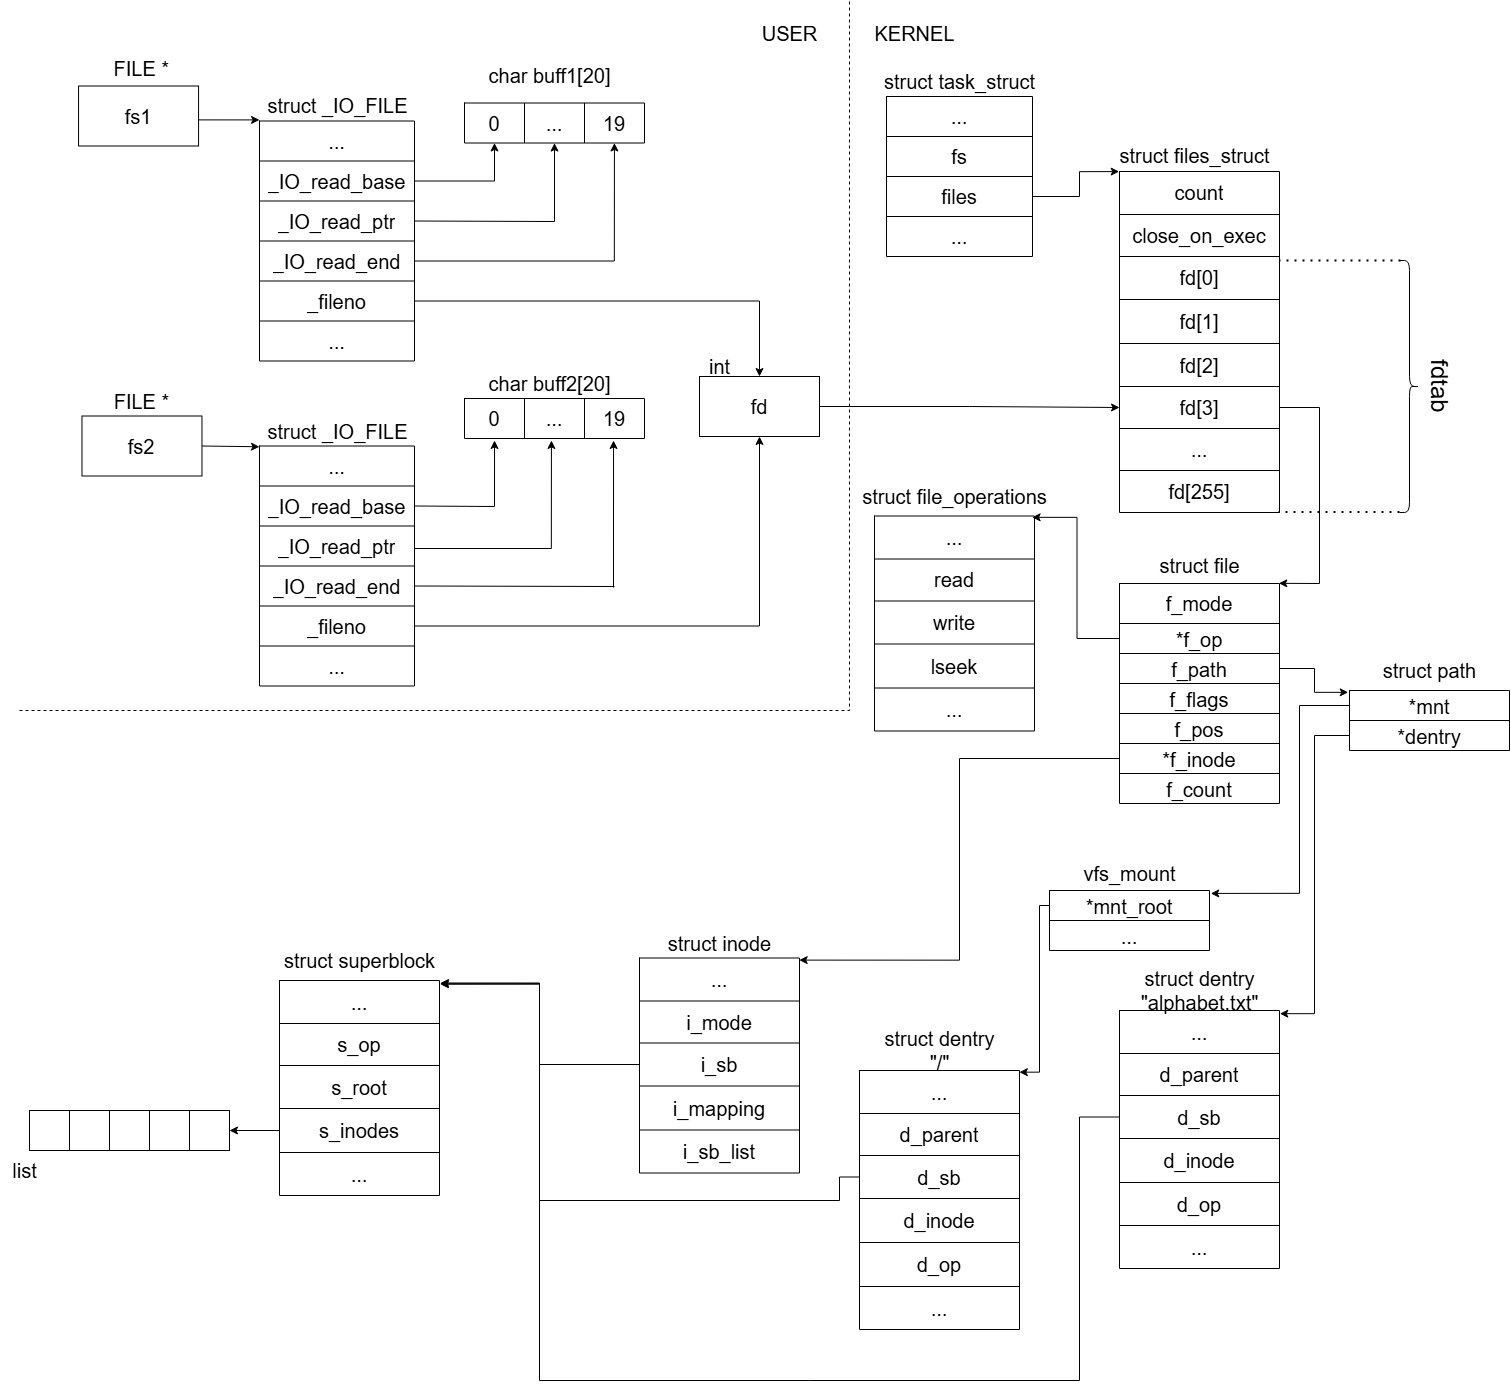
\includegraphics[width=\textwidth]{img/11}
	\caption{Связь структур в файловой подсистеме Linux, используемых в первой программе}
    \label{fig:prog1}
\end{figure}\newpage

\newpage
\clearpage

\section{Вторая программа}

\subsection{Однопоточная программа}

\captionsetup{singlelinecheck = false, justification=raggedright}
\lstinputlisting[label=lst:author, caption=Вторая программа, language=c]{src/second.c}

\begin{figure}[H]
	\centering
	
\includegraphics[width=\textwidth]{img/2-1}
	\caption{Результат работы второй программы}
\end{figure}

\subsection{Анализ результата работы однопоточной программы}
Во второй программе посредством двух вызовов \texttt{open()} файл\\ <<abc.txt>>
дважды открывается только для чтения (\texttt{O\_RDONLY}), создаются два дескриптора открытого файла (\texttt{fd1} и \texttt{fd2}), которым присваиваются значения 3 и 4 соответственно. Создаются два объекта структуры \texttt{struct file}, ссылающиеся на один и тот же объект \texttt{struct~inode}. Так как объекты \texttt{struct file} разные и их поля \texttt{f\_pos} изменяются независимо, то для каждого файлового дескриптора произойдет полное чтение файла и каждый символ будет выведен по два раза.

\subsection{Многопоточная программа}

\captionsetup{singlelinecheck = false, justification=raggedright}
\lstinputlisting[label=lst:author2, caption=Вторая программа с 1-м дополнительным потоком, language=c]{src/second_thr.c}

\begin{figure}[H]
	\centering
	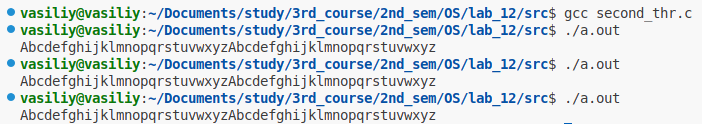
\includegraphics[width=\textwidth]{img/2-3}
	\caption{Результат работы второй программы с 1-м дополнительным потоком}
\end{figure}


\captionsetup{singlelinecheck = false, justification=raggedright}
\lstinputlisting[label=lst:author, caption=Вторая программа с 2-мя дополнительными потоками, language=c]{src/second_thr2.c}

\begin{figure}[H]
	\centering
	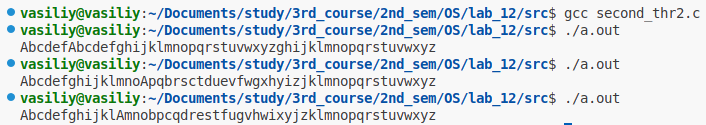
\includegraphics[width=\textwidth]{img/2-2}
	\caption{Результат работы второй программы с 2-мя дополнительными потоками}
\end{figure}

\newpage

\subsection{Анализ результата работы многопоточной программы}
При многопоточной реализации алфавит также будет выведен два раза, однако
порядок вывода символов заранее предсказать невозможно. В случае с главным и дополнительным потоком дополнительный поток начинает выполнение позже главного, так как на его создание затрачивается время.

\section{Вторая программа (другой вариант)}

\subsection{Однопоточная программа}

\captionsetup{singlelinecheck = false, justification=raggedright}
\lstinputlisting[label=lst:author2, caption=Вторая программа (другой вариант), language=c]{src/third.c}

\begin{figure}[H]
	\centering
	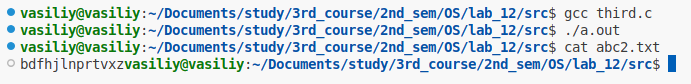
\includegraphics[width=\textwidth]{img/22-1}
	\caption{Результат работы второй программы (другой вариант)}
\end{figure}

\subsection{Анализ результата однопоточной программы}

Во второй программе с использованием \texttt{open()} файл дважды открывается на чтение и запись (O\_RDWR).
Возвращаются два дескриптора открытого файла (со значениями 3 и 4) системной таблицы открытых файлов процесса.
При каждом открытии файла создается новый объект \texttt{struct file}, который ссылается на один и тот же объект
\texttt{struct inode}. Так как объекты структур разные и их поля изменяются независимо,
то при записи всех четных букв они будут перезаписаны нечетными, так как поля \texttt{f\_pos}
изменяются независимо у обоих объектов.

\clearpage

\subsection{Многопоточная программа}

\captionsetup{singlelinecheck = false, justification=raggedright}
\lstinputlisting[label=lst:author4, caption=Вторая программа (другой вариант) с 1-м дополнительным потоком, language=c]{src/third_thr.c}

\begin{figure}[H]
	\centering
	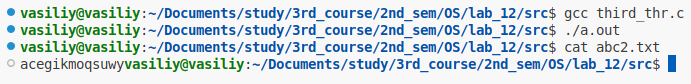
\includegraphics[width=\textwidth]{img/22-3}
	\caption{Результат работы второй программы (другой вариант) с 1-м дополнительным потоком}
\end{figure}

\captionsetup{singlelinecheck = false, justification=raggedright}
\lstinputlisting[label=lst:author3, caption=Вторая программа (другой вариант) с 2-мя дополнительными потоками, language=c]{src/third_thr2.c}

\begin{figure}[H]
	\centering
	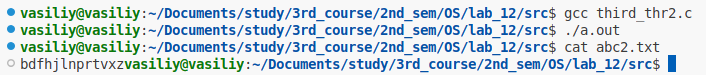
\includegraphics[width=\textwidth]{img/22-2}
	\caption{Результат работы второй программы (другой вариант) с 2-мя дополнительными потоками}
\end{figure}

\subsection{Анализ результата работы многопоточной программы}

Как и в однопоточной программе, в данном случае создаются два независимых экземпляра структуры.
Однако результат выполнения зависит от порядка планирования потоков.
Если поток, записывающий четные символы, первым начнет писать в файл данные,
а затем будет писать поток с нечетными символами, последний перезапишет все четные символы на нечетные символы.

\subsection{Связь структур}
\begin{figure}[H]
	\centering
	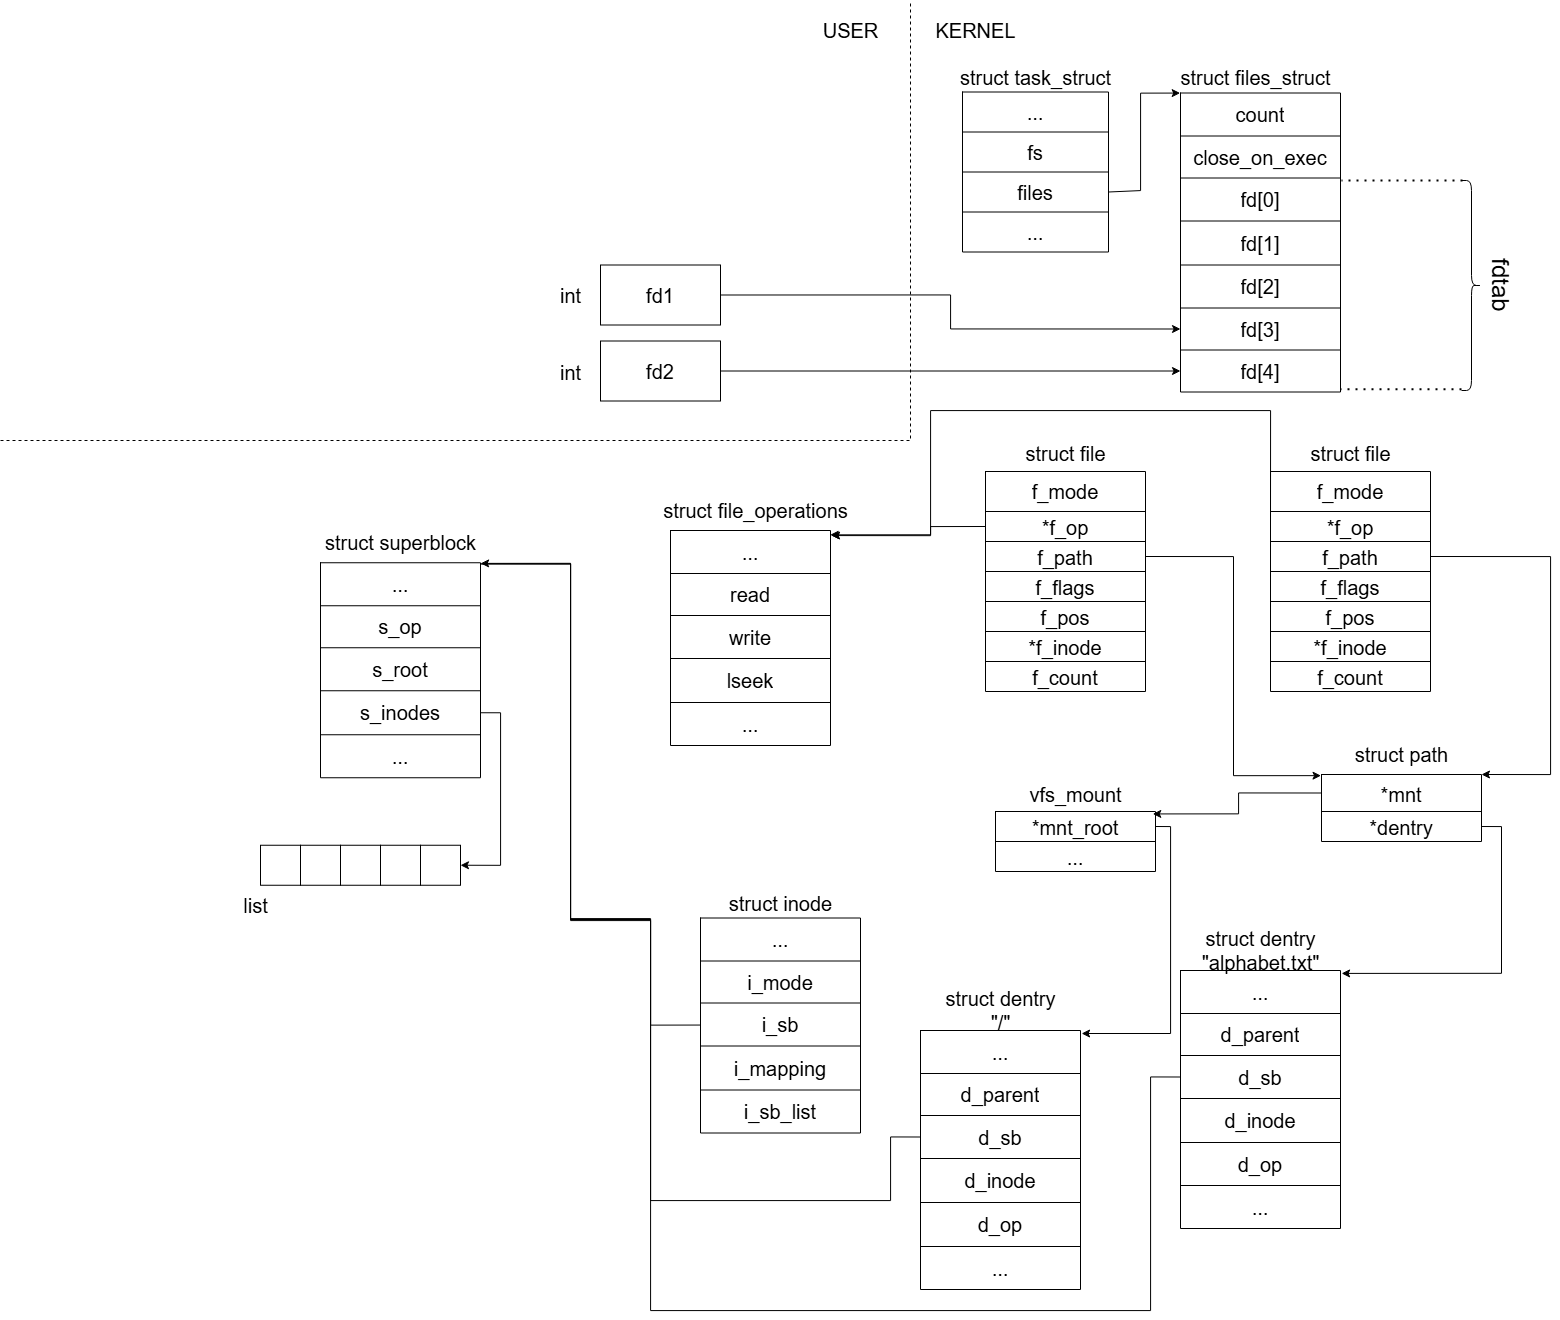
\includegraphics[width=\textwidth]{img/22}
	\caption{Связь структур в файловой подсистеме Linux, используемых во второй программе}
    \label{fig:prog2}
\end{figure}\newpage

\newpage

\section{Третья программа}

\captionsetup{singlelinecheck = false, justification=raggedright}
\lstinputlisting[label=lst:lst-1, caption=Описание структуры stat, language=c]{structs/stat.txt}

\subsection{Однопоточная программа}
\captionsetup{singlelinecheck = false, justification=raggedright}
\lstinputlisting[label=lst:lst-5, caption=Третья программа с fopen, language=c]{src/fopen.c}


\captionsetup{singlelinecheck = false, justification=raggedright}
\lstinputlisting[label=lst:lst-6, caption=Результат работы третьей программы с open, language=bash]{structs/3-1.txt}


\subsection{Анализ результатов однопоточной программы}

В третьей программе с использованием \texttt{fopen()} файл дважды открывается на запись (опция <<w>>). Так же, как и во второй программе, создаются два файловых дескриптора (со значениями 3 и 4), на которые ссылаются объекты структуры \texttt{FILE} (\texttt{fs1, fs2}). По умолчанию используется
буферизация, при которой запись в файл из буфера происходит когда буфер заполнен, либо когда вызывается \texttt{fflush}, либо \texttt{fclose}.

В данном случае, с помощью вывода полей структуры \texttt{struct stat}, можно наблюдать, что запись происходит при вызове \texttt{fclose()}. До
вызовов \texttt{fclose()} в цикле в файл записываются буквы латинского
алфавита с помощью поочередной передачи функции \texttt{fprintf()} дескрипторов, при этом изменяется только поле \texttt{f\_pos} соответствующего дескриптора.

При вызове \texttt{fclose(fs1)} четные буквы алфавита записываются в файл.
При вызове \texttt{fclose(fs2)}, так как поле \texttt{f\_pos}
соответствующей структуры \texttt{struct file} изменялось независимо, запись в файл
произойдет с начала файла, и записанные ранее символы перезапишутся нечетными буквами алфавита. Так как буферы содержали одинаковое количество символов, данные первой
записи утеряны.

% В третьей программе с использованием open() результат аналогичный, поскольку установлен флаг \texttt{O\_WRONLY}. Схема связи структур, используемых в третьей программе с open() совпадает с рисунком 6.

% Проблема решается добавлением флага \texttt{O\_APPEND} в программу с open() или изменением опции <<w>> на опцию <<a>> в программе с fopen().

Таким образом, при буферизованном вводе-выводе все данные и при чтении, и при записи пишутся сначала в буфер, а только после этого в файл. В случае небуферизованного ввода-вывода данные напрямую записываются в файл или считываются из него без промежуточного буферирования.

\subsection{Многопоточная программа}
\captionsetup{singlelinecheck = false, justification=raggedright}
\lstinputlisting[label=lst:lst-5, caption=Третья программа с fopen с 1-м дополнительным потоком, language=c]{src/fopen_thr.c}

\captionsetup{singlelinecheck = false, justification=raggedright}
\lstinputlisting[label=lst:lst-6, caption=Результат работы третьей программы с fopen с 1-м дополнительным потоком, language=bash]{structs/3-3.txt}


\captionsetup{singlelinecheck = false, justification=raggedright}
\lstinputlisting[label=lst:lst-5, caption=Третья программа с fopen с 2-мя дополнительными потоками, language=c]{src/fopen_thr2.c}

\captionsetup{singlelinecheck = false, justification=raggedright}
\lstinputlisting[label=lst:lst-6, caption=Результат работы третьей программы с open с 2-мя дополнительными потоками, language=bash]{structs/3-2.txt}


\subsection{Анализ результатов многопоточной программы}
Аналогично однопоточной программе здесь с использованием \newline \texttt{fopen()} файл дважды открывается на запись и создаются два файловых дескриптора (со значениями 3 и 4), на которые ссылаются объекты структуры \texttt{FILE} (\texttt{fs1, fs2}). Особенность буферизованного вывода приводит к тому, что данные сначала накапливаются в отдельных буферах каждого потока, а запись в файл происходит только при вызове \texttt{fclose()} или \texttt{fflush()}, или заполнении буфера.

% Статистика файла (st_ino, st_size, pos) показывает интересную динамику: хотя потоки уже записали данные в свои буферы (что отражается в позиции pos), реальный размер файла (st_size) остаётся нулевым до момента фактической записи на диск при закрытии. Это наглядно демонстрирует работу буферизации.

\clearpage

\subsection{Связь структур}

\begin{figure}[H]
	\centering
	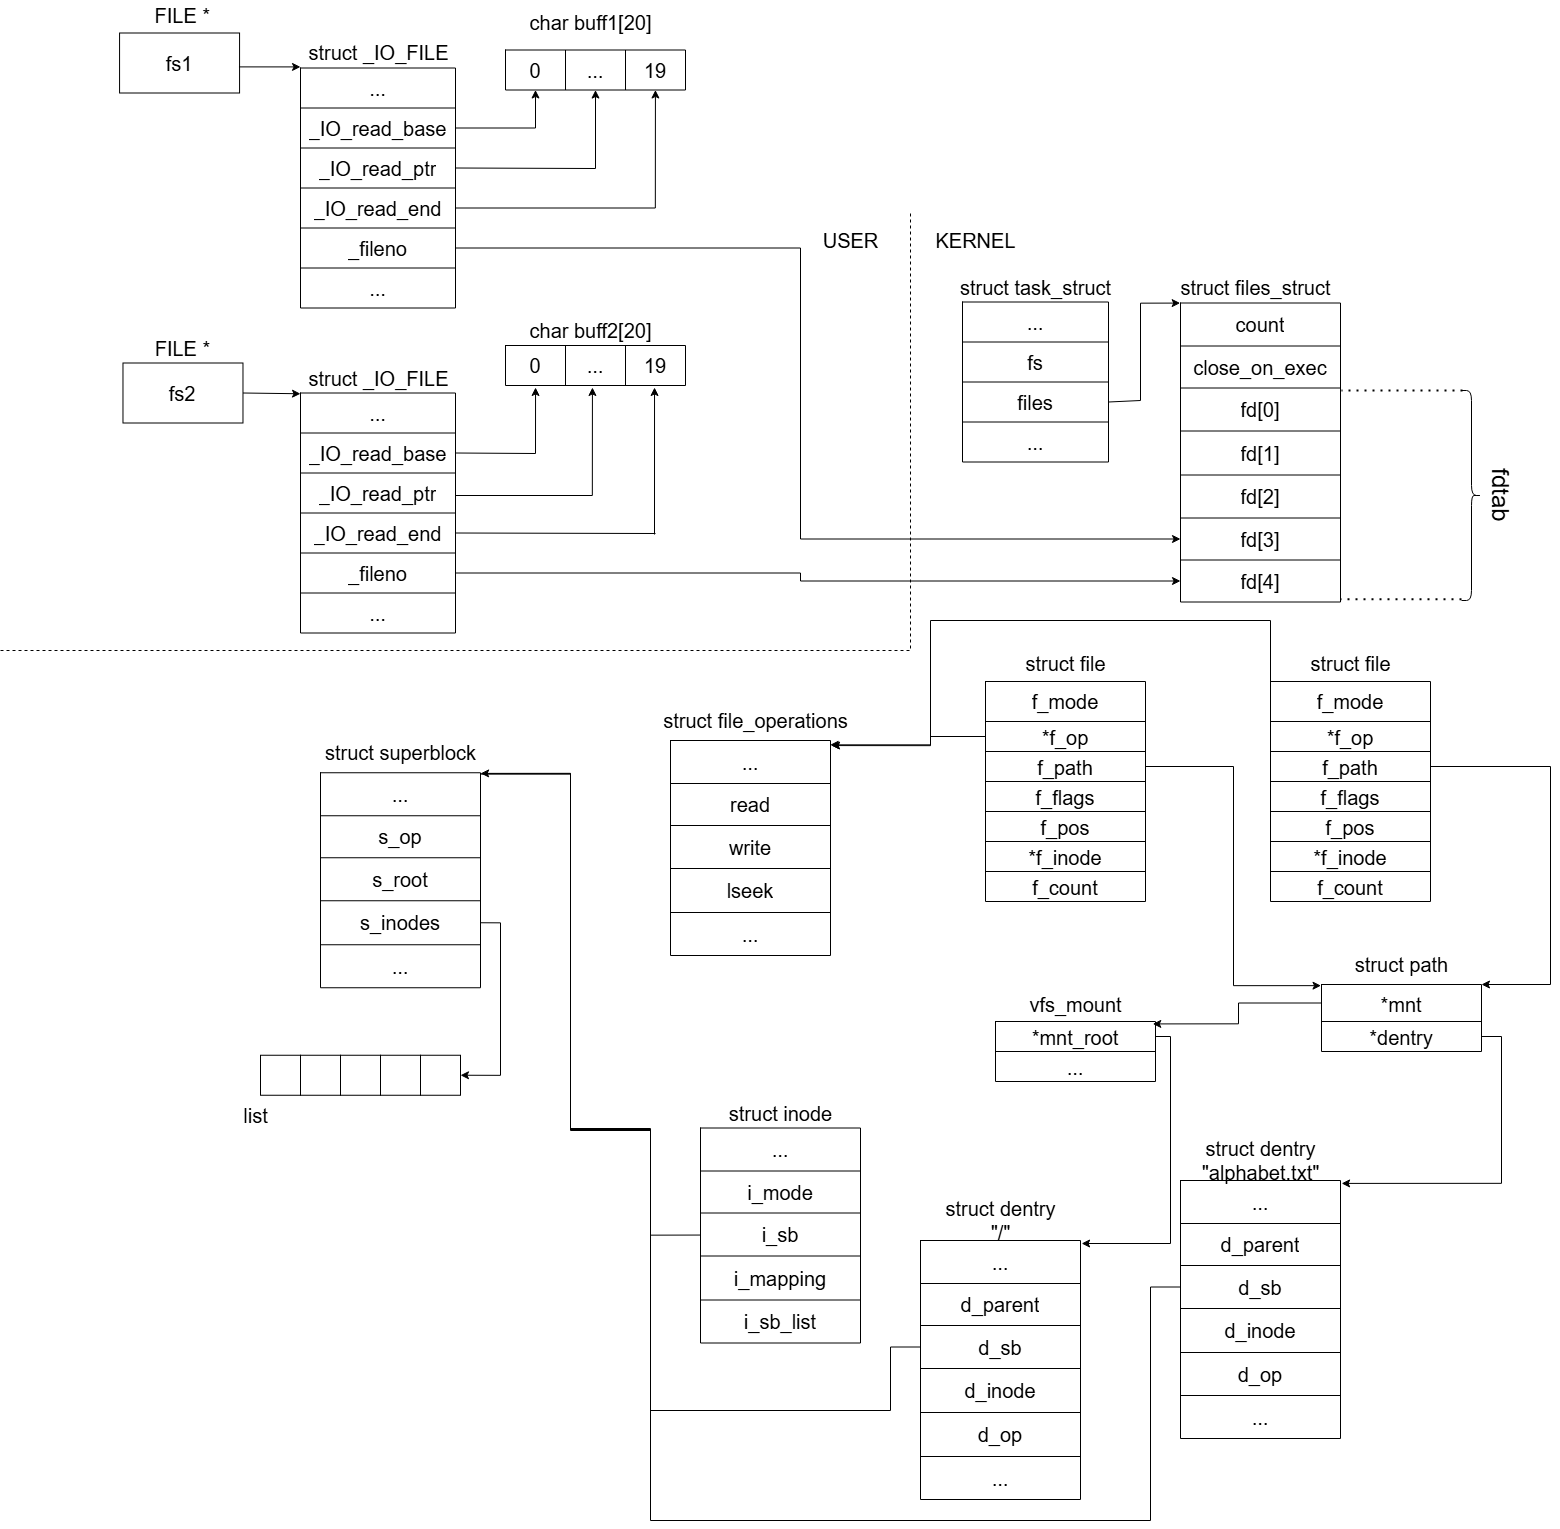
\includegraphics[width=\textwidth]{img/33}
	\caption{Связь структур в файловой подсистеме Linux, используемых в третьей программе с fopen}
    \label{fig:prog3}
\end{figure}



\clearpage


\section{Варианты решения проблемы синхронизации}
Для решения проблемы можно использовать несколько подходов:
\begin{itemize}
    \item Режим дописывания ("a" или O\_APPEND) вместо перезаписи ("w") гарантирует  добавление в конец файла;
    \item Явная синхронизация потоков через средства взаимоисключения;
    \item Принудительный сброс буфера (fflush) после каждой операции записи.
\end{itemize}
